\documentclass{beamer}
\usetheme{Singapore}

\usepackage{enumerate}
\usepackage{fontawesome}
\usepackage[round]{natbib}
\usepackage{tikz}
\usepackage{listings}
\usetikzlibrary{shapes,snakes,arrows.meta,shapes.arrows,backgrounds}

\lstdefinelanguage{scala}{
  morekeywords={%
          abstract,case,catch,class,def,do,else,extends,%
          false,final,finally,for,forSome,if,implicit,import,lazy,%
          match,new,null,object,override,package,private,protected,%
          return,sealed,super,this,throw,trait,true,try,type,%
          val,var,while,with,yield},
  otherkeywords={=>,<-,<\%,<:,>:,\#,@},
  sensitive=true,
  morecomment=[l]{//},
  morecomment=[n]{/*}{*/},
  morestring=[b]",
  morestring=[b]',
  morestring=[b]"""
}[keywords,comments,strings]

% activate the language and predefine settings
\lstset{language=Scala}

\title{T\'{e}cnicas de Programa\c c\~{a}o 2}

\subtitle{Implementa\c c\~{a}o da Linguagem Oberon-0}

\author{Rodrigo Bonif\'{a}cio}

\begin{document}

\begin{frame}
 \titlepage
\end{frame}

\section{Oberon}

\begin{frame}

  \emph{Oberon-0 is an imperative language designed by Niklaus Wirth}~\citep{wirth1996compiler,ldta-scp} \pause

  \begin{block}{Features}
     \begin{itemize}
      \item declara\c c\~{o}es: constantes e vari\'{a}veis
      \item tipos: primitivos (bool, int, \ldots), arrays, records, sets
      \item express\~{o}es: relacionais, aritim\'{e}ticas, booleanas, \ldots
      \item comandos: assignment, condicionais, repeti\c c\~{a}o
      \item procedimentos: passagem por valor e por refer\^{e}ncia  
     \end{itemize}
  \end{block}
  \pause
  

  \begin{center}
  Explorada em um desafio sobre novas tecnologias para
     \emph{meta programa\c c\~{a}o}~\citep{ldta-scp}. 
  \end{center}
  
\end{frame}

\begin{frame}
  \begin{quotation}
    ``We wanted [to explore] a language with a
    reasonable level of complexity but not a large language that
    had many features that would not illustrate the power of the tools''
  \end{quotation}
  \begin{flushright}
    \citep{ldta-scp}
  \end{flushright} \pause

  Vamos explorar as constru\c c\~{o}es da linguagem Scala e
  algumas t\'{e}cnicas para o
  {\color{blue}desenho} e {\color{blue}evolu\c c\~{a}o}
  de uma implementa\c c\~{a}o de Oberon-0\pause---cuja implementa\c c\~{a}o inicial seguiu o desafio de programa\c c\~{a}o proposto por  \citet{ldta-scp}.
\end{frame}

\begin{frame}
    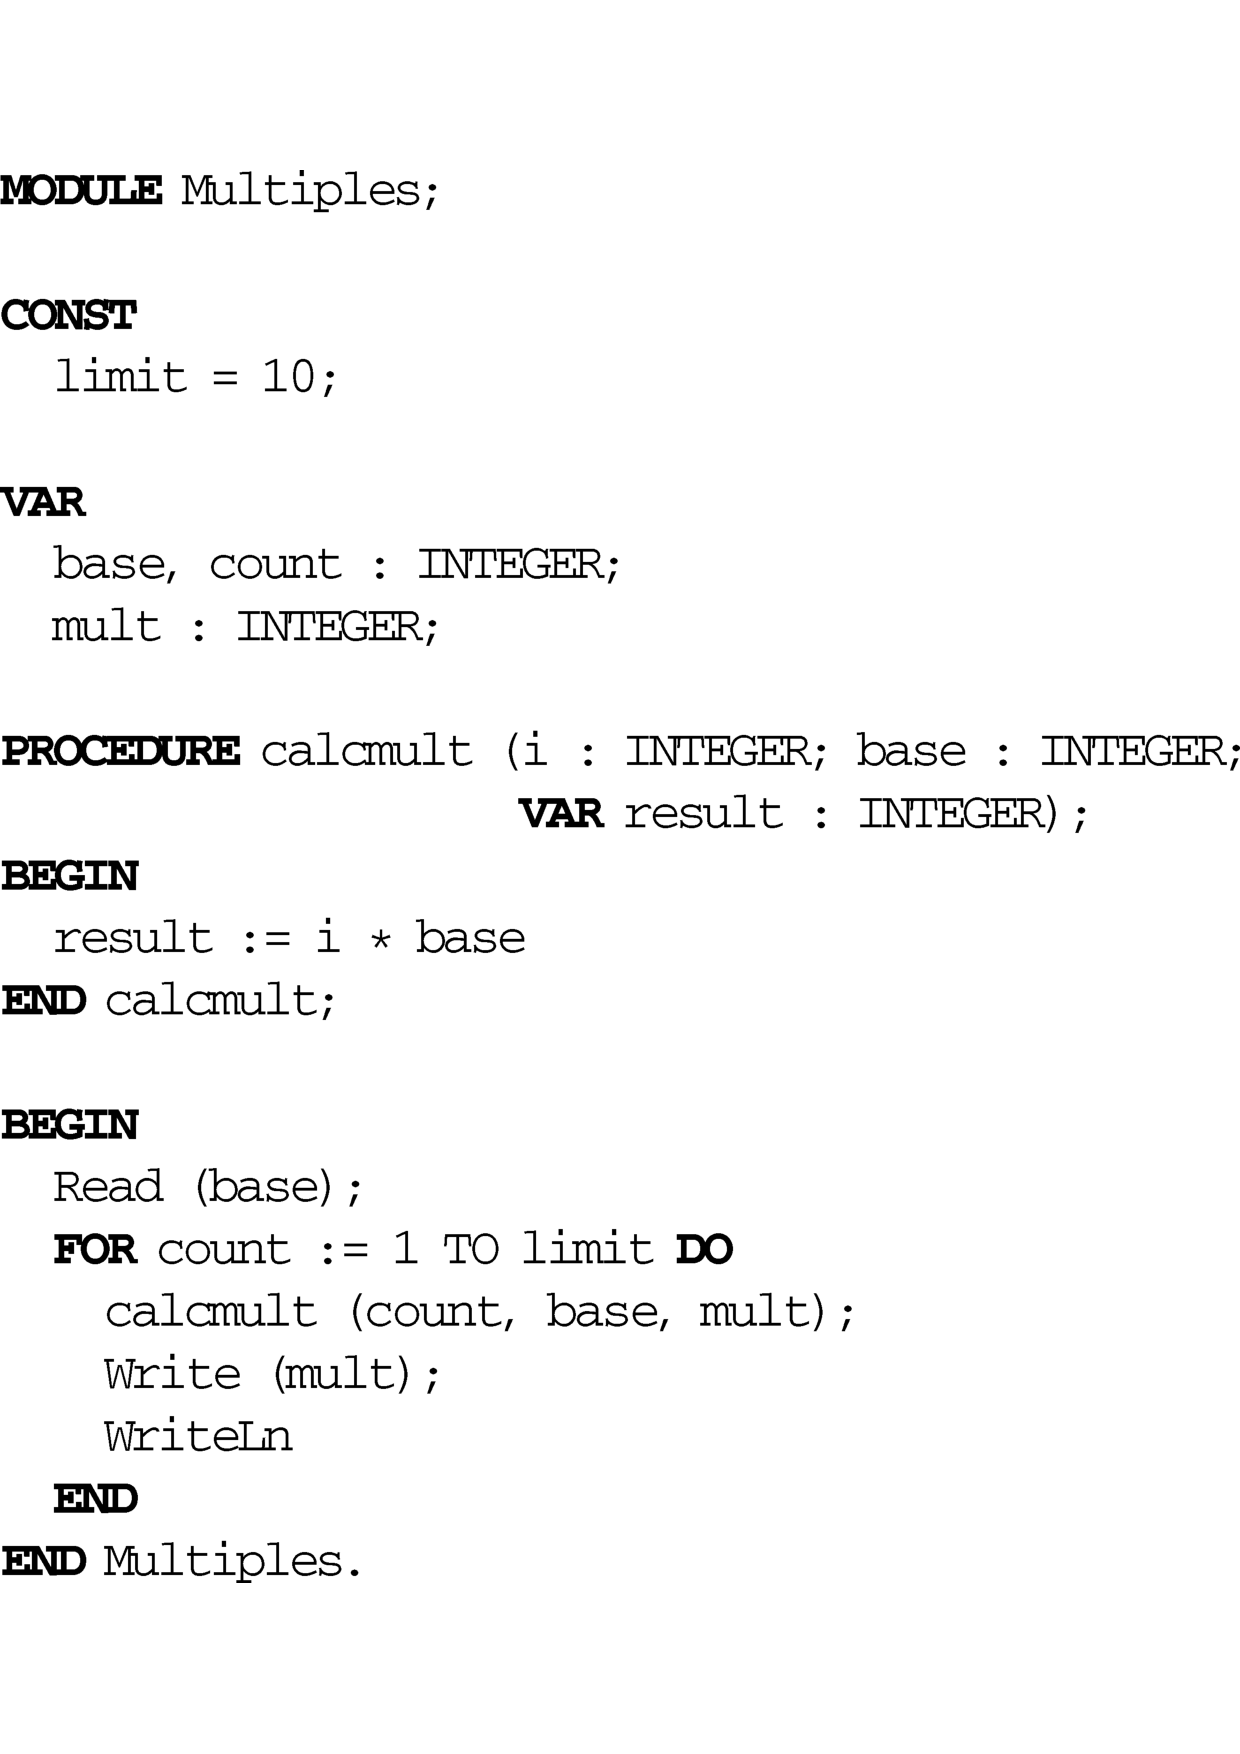
\includegraphics[scale=0.27]{imagens/code.pdf}
\end{frame} 

\section{Implementa\c c\~{a}o de Linguagens}

\begin{frame}
  \begin{center}
\huge{Implementa\c c\~{a}o de Linguagens \\ \pause  \faQuestionCircle}
\end{center}
\end{frame}

  \begin{frame}
  \frametitle{Estilo Arquitetural}

  \begin{figure}
    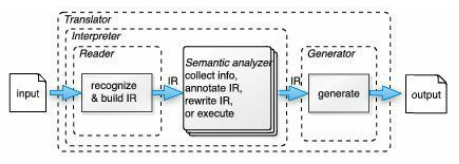
\includegraphics[scale=0.5]{imagens/arquitetura.png}
  \end{figure}
  \begin{center}
     {\color{blue}Multistage Pipeline} \citep{lip-book}
  \end{center}
  \pause
  
  \begin{block}{Componentes da Implementa\c c\~{a}o Oberon-0}
    \begin{enumerate}
     \item parser 
     \item an\'{a}lise sem\^{a}ntica
     \item (otimiza\c c\~{a}o de c\'{o}digo)?
     \item \{ interpreta\c c\~{a}o $\mid$ tradu\c c\~{a}o\}  
    \end{enumerate}
  \end{block}
\end{frame}

\section{Parser}
  
\begin{frame}
\huge{Parser} 
\end{frame}
\begin{frame}
  \frametitle{Parser}

  Dois sub-componentes: {\color{blue}analisador l\'{e}xico} e
  {\color{blue}analisador sint\'{a}tico}. O parser busca reconhecer
  um programa em uma determinada linguagem, e produzir
  como sa\'{i}da uma representa\c c\~{a}o intermedi\'{a}ria
  (tipicamente uma AST). 

  \pause
  \begin{block}{Diferentes formas de implementa\c c\~{a}o}
\begin{small}
  \begin{itemize}
   \item \emph{from scratch}
   \item usando uma biblioteca de combinadores
   \item usando um gerador de parser (Bison/YACC, BNFC, {\bf ANTLR}, \ldots)  
  \end{itemize}
\end{small}
\end{block}
  
\end{frame}

\begin{frame}[fragile]
  \frametitle{ANTLR (Gerador de Parser)}
  \begin{figure}
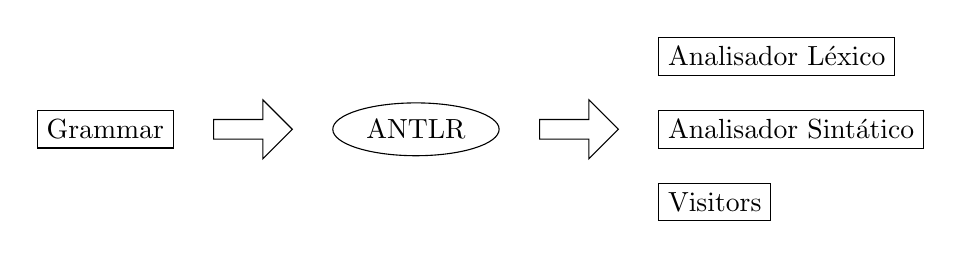
\begin{tikzpicture}[scale=2]
    \tikzstyle{ann} = [draw=none,fill=none,left, nodes={rectangle, draw}]]
    \matrix[nodes={draw}, row sep=0.3cm,column sep=0.5cm,
    column 1/.style={anchor=west},
    column 2/.style={anchor=west},
    column 3/.style={anchor=west},
    column 4/.style={anchor=west},
    column 5/.style={anchor=west}] { 
                                & &                         & & \node[rectangle] {Analisador L\'{e}xico};   \\
    \node[rectangle] {Grammar}; & \node[single arrow, minimum height=1cm]{}; & \node[ellipse] {ANTLR}; & \node[single arrow, minimum height=1cm]{}; & \node[rectangle] {Analisador Sint\'{a}tico};\\
                                & &                         & & \node[rectangle] {Visitors};   \\
    };
\end{tikzpicture}
\end{figure}
  \pause
  \vskip+1.5em
\begin{itemize}
\item Precisamos apenas transformar o resultado do parser
  ANTLR em uma representa\c c\~{a}o intermedi\'{a}ria (e independente
  do ANTLR). Justificativa: podemos alterar a gram\'{a}tica / estrat\'{e}gia
  de implementa\c c\~{a}o do parser sem quebrar as demais fases do
  pipeline.
\end{itemize}
\end{frame}

\begin{frame}
  \frametitle{Outra abstra\c c\~{a}o da arquitetura}
  \begin{figure}
    \includegraphics[scale=0.3]{imagens/parser.pdf}
  \end{figure}
\end{frame}

\begin{frame}
  \frametitle{\'{A}rvore Sint\'{a}tica Abstrata}

  Representa\c c\~{a}o de um m\'{o}dulo de um
  programa mais f\'{a}cil de ser manipulada
  em algum est\'{a}gio de um compilador ou
  interpretador.

  \begin{block}{Cen\'{a}rios de uso de uma AST}
    \begin{itemize}
     \item verifica\c c\~{a}o de tipos
     \item c\'{a}lculo de m\'{e}tricas
     \item refatoramento de c\'{o}digo   
     \item interpreta\c c\~{a}o de programas
     \item gera\c c\~{a}o direta de c\'{o}digo  
    \end{itemize} 
  \end{block}  \pause

  Alguns tipos de an\'{a}lise / transforma\c c\~{o}es
  de programas s\~{a}o vi\'{a}veis apenas em
  representa\c c\~{o}es mais baixo n\'{i}vel
  (exemplo: three-address code)

\end{frame}

\section{Interpretador}

\begin{frame}
\huge{Interpretador}
\end{frame}

\begin{frame}
  \begin{itemize}
  \item Oberon \'{e} uma linguagem {\color{blue}imperativa}\pause: modelo
  computacional corresponde a uma sequencia de comandos
  que atualizam o {\color{blue}estado do programa}. \pause

  \item O estado do programa corresponde aos {\color{blue}mapeamentos} entre
  vari\'{a}veis e constantes (tanto globais quanto locais)
  em valores (express\~{o}es)\pause---em um determinado instante.
 \end{itemize} 
\end{frame}

\begin{frame}
  \begin{block}{Representa\c c\~{a}o do Estado}
    Classe \texttt{Environment} contendo: \pause
    \begin{itemize}
     \item \texttt{globals: Map[String, Exp]} com as vari\'{a}veis globais
     \item \texttt{locals: Stack[Map[String, Exp]]} com as vari\'{a}veis locais
     \item \texttt{procedures: List[Procedure]} com as declara\c c\~{o}es de procedimentos   
    \end{itemize} \pause
    e opera\c c\~{o}es para indicar que um procedimento foi chamado, que uma
    procedimento retornou (concluiu a execu\c c\~{a}o) e que uma atribui\c c\~{a}o
    foi realizada. 
  \end{block}  
\end{frame}

\begin{frame}
  \begin{block}{Interpreta\c c\~{a}o de um Programa Oberon}
    \begin{enumerate}[(a)]
     \item mapear as constantes globais no ambiente
     \item mapear as vari\'{a}veis globais no ambiente
     \item mapear os procedimentos no ambiente  
     \item interpretar o bloco de comandos principal \pause
    \end{enumerate}
  \end{block}
  
  \begin{itemize}
   \item solu\c c\~{a}o atual: {\color{blue}visitor} + {\color{blue}pattern matching}  
  \end{itemize}
\end{frame}

\begin{frame}[fragile]
  \begin{lstlisting}
trait OberonVisitor {
  type T
  var result : T = _
  def visit(module: OberonModule) : Unit
  def visit(constant: Constant) : Unit
  def visit(variable: VariableDeclaration) : Unit
  def visit(procedure: Procedure) : Unit
  def visit(arg: FormalArg) : Unit
  def visit(exp: Expression) : Unit
  def visit(stmt: Statement) : Unit
  def visit(aType: Type) : Unit
}
  \end{lstlisting} 
\end{frame}

\begin{frame}[fragile]
\begin{scriptsize}  
  \begin{lstlisting}
case class OberonModule(
   name: String,
   constants: List[Constant],
   variables: List[VariableDeclaration],
   procedures: List[Procedure],
   stmt: Option[Statement]
  )
{
  def accept(v: OberonVisitor): Unit = v.visit(this)
}
  \end{lstlisting}
\end{scriptsize}  
\end{frame}


\begin{frame}
  \begin{block}{Observa\c c\~{a}o}
   \begin{itemize}
   \item Em cada chamada de procedimento, precisamos:
     \begin{enumerate}[(i)]
      \item associar os argumentos atuais com os argumentos formais \faStar
      \item atualizar a pilha com as declara\c c\~{o}es locais do procedimento
      \item executar o bloco de comandos do procedimento. \pause
     \end{enumerate}   
    \item  Quando retornamos de um procedimento, precisamos {\color{blue}liberar}
     essas vari\'{a}veis locais.  
  \end{itemize}
 \end{block} 
\end{frame}

\begin{frame}[fragile]
  \begin{scriptsize}
    \begin{lstlisting}
def call(p: Procedure, args: List[Expression]): Unit = {
  p.args.map(formal => formal.name)
        .zip(args)
        .foreach(pair => env.setLocalVariable(pair._1, pair._2))

  p.constants.foreach(c => env.setLocalVariable(c.name, c.exp))
  p.variables.foreach(v => env.setLocalVariable(v.name, Undef()))
}
    \end{lstlisting}  
  \end{scriptsize}
\end{frame}

\begin{frame}[t, allowframebreaks]
  \frametitle{Refer\^{e}ncias}
  \bibliographystyle{abbrvnat}
 \bibliography{referencias}
\end{frame}

\begin{frame}
\titlepage
\end{frame}

\end{document}
